% Graphic for TeX using PGF
% Title: /home/FatLord/Diagrama4.dia
% Creator: Dia v0.97.3
% CreationDate: Wed Oct  7 22:16:58 2015
% For: FatLord
% \usepackage{tikz}
% The following commands are not supported in PSTricks at present
% We define them conditionally, so when they are implemented,
% this pgf file will use them.
\ifx\du\undefined
  \newlength{\du}
\fi
\setlength{\du}{15\unitlength}
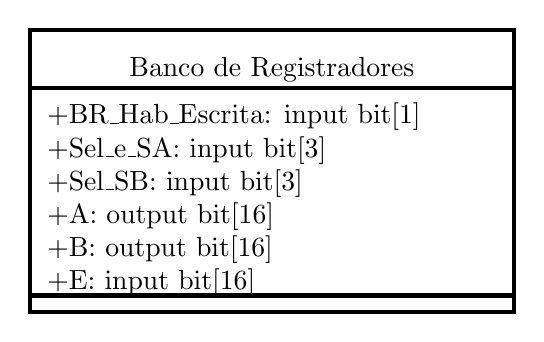
\begin{tikzpicture}
\pgftransformxscale{1.000000}
\pgftransformyscale{-1.000000}
\definecolor{dialinecolor}{rgb}{0.000000, 0.000000, 0.000000}
\pgfsetstrokecolor{dialinecolor}
\definecolor{dialinecolor}{rgb}{1.000000, 1.000000, 1.000000}
\pgfsetfillcolor{dialinecolor}
\pgfsetlinewidth{0.100000\du}
\pgfsetdash{}{0pt}
\definecolor{dialinecolor}{rgb}{1.000000, 1.000000, 1.000000}
\pgfsetfillcolor{dialinecolor}
\fill (15.800000\du,11.450000\du)--(15.800000\du,12.850000\du)--(27.465000\du,12.850000\du)--(27.465000\du,11.450000\du)--cycle;
\definecolor{dialinecolor}{rgb}{0.000000, 0.000000, 0.000000}
\pgfsetstrokecolor{dialinecolor}
\draw (15.800000\du,11.450000\du)--(15.800000\du,12.850000\du)--(27.465000\du,12.850000\du)--(27.465000\du,11.450000\du)--cycle;
% setfont left to latex
\definecolor{dialinecolor}{rgb}{0.000000, 0.000000, 0.000000}
\pgfsetstrokecolor{dialinecolor}
\node at (21.632500\du,12.400000\du){Banco de Registradores };
\definecolor{dialinecolor}{rgb}{1.000000, 1.000000, 1.000000}
\pgfsetfillcolor{dialinecolor}
\fill (15.800000\du,12.850000\du)--(15.800000\du,17.850000\du)--(27.465000\du,17.850000\du)--(27.465000\du,12.850000\du)--cycle;
\definecolor{dialinecolor}{rgb}{0.000000, 0.000000, 0.000000}
\pgfsetstrokecolor{dialinecolor}
\draw (15.800000\du,12.850000\du)--(15.800000\du,17.850000\du)--(27.465000\du,17.850000\du)--(27.465000\du,12.850000\du)--cycle;
% setfont left to latex
\definecolor{dialinecolor}{rgb}{0.000000, 0.000000, 0.000000}
\pgfsetstrokecolor{dialinecolor}
\node[anchor=west] at (15.950000\du,13.550000\du){+BR\_Hab\_Escrita: input bit\ensuremath{[}1\ensuremath{]}};
% setfont left to latex
\definecolor{dialinecolor}{rgb}{0.000000, 0.000000, 0.000000}
\pgfsetstrokecolor{dialinecolor}
\node[anchor=west] at (15.950000\du,14.350000\du){+Sel\_e\_SA: input bit\ensuremath{[}3\ensuremath{]}};
% setfont left to latex
\definecolor{dialinecolor}{rgb}{0.000000, 0.000000, 0.000000}
\pgfsetstrokecolor{dialinecolor}
\node[anchor=west] at (15.950000\du,15.150000\du){+Sel\_SB: input bit\ensuremath{[}3\ensuremath{]}};
% setfont left to latex
\definecolor{dialinecolor}{rgb}{0.000000, 0.000000, 0.000000}
\pgfsetstrokecolor{dialinecolor}
\node[anchor=west] at (15.950000\du,15.950000\du){+A: output bit\ensuremath{[}16\ensuremath{]}};
% setfont left to latex
\definecolor{dialinecolor}{rgb}{0.000000, 0.000000, 0.000000}
\pgfsetstrokecolor{dialinecolor}
\node[anchor=west] at (15.950000\du,16.750000\du){+B: output bit\ensuremath{[}16\ensuremath{]}};
% setfont left to latex
\definecolor{dialinecolor}{rgb}{0.000000, 0.000000, 0.000000}
\pgfsetstrokecolor{dialinecolor}
\node[anchor=west] at (15.950000\du,17.550000\du){+E: input bit\ensuremath{[}16\ensuremath{]}};
\definecolor{dialinecolor}{rgb}{1.000000, 1.000000, 1.000000}
\pgfsetfillcolor{dialinecolor}
\fill (15.800000\du,17.850000\du)--(15.800000\du,18.250000\du)--(27.465000\du,18.250000\du)--(27.465000\du,17.850000\du)--cycle;
\definecolor{dialinecolor}{rgb}{0.000000, 0.000000, 0.000000}
\pgfsetstrokecolor{dialinecolor}
\draw (15.800000\du,17.850000\du)--(15.800000\du,18.250000\du)--(27.465000\du,18.250000\du)--(27.465000\du,17.850000\du)--cycle;
\end{tikzpicture}
